\section{การนำเสนอภาพ}

\hspace{1cm} ก่อนจะนำเสรอขั้นตอนวิธีเชิวตัวเลขชนิดใหม่จะขอกล่าวถึงการนำเสนอภาพโดยเชิงคณิตศาสตร์ ดังนี้

\subsection{การนำเสนอภาพเฉดเทา}

\hspace{1cm} กำหนดให้ $I$ แทนภาพเฉดเทา (grayscale image) นิยามโดย
\begin{align*}
    I : \Omega \subset \mathbb{R}^2 \rightarrow V \subset [0,\infty)	
\end{align*}

 เป็นฟังก์ชันต่อเนื่อง โดยที่ $ \mathbf{x} = (x,y) \in \Omega $ แทนพิกัดทางกายภาพ (physical position) ของภาพ $ I(\mathbf{x}) \in V $ แทนระดับความเข้มของภาพ (image intensity) ที่ $ \mathbf{x} $ และ $ \Omega $ แทนโดเมนของภาพซึ่งเป็นรูปร่างสีเหลี่ยม ซึ่งในที่นี้สามารถสมมติได้โดยไม่เสียหลักการสำคัญว่า $ \Omega = [1,n]^2 $ และ $ V = [0,1] $ เมื่อ $n>1$ เป็นจำนวนเต็มบวก 

\begin{figure}[H]
    \centering
    \begin{subfigure}{0.8\linewidth}
        \centering
        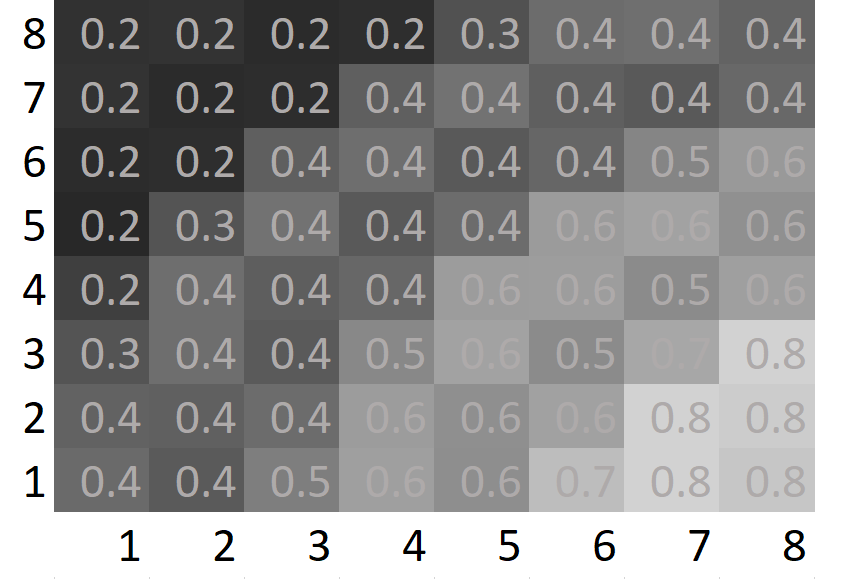
\includegraphics[width=0.45\linewidth]{image/grayscale-explain.png}
    \end{subfigure}
    \caption{ตัวอย่างภาพเฉดเทาที่แสดงระดับความเข้มของภาพในแต่ละระดับ}
    \label{figure:grayscale-explain}
\end{figure}

\hspace{1cm} จากภาพ \ref{figure:grayscale-explain} สังเกตว่าที่ค่าความเข้มของภาพเข้าใกล้ 0 จะให้สีเป็นลักษณะสีดำ ดังเช่นบริเวณที่พิกัดทางกายภาพเป็น (4,8) และเมื่อค่าความเข้มของสีเข้าใกล้ 1 จะให้สีที่มีลักษณะเป็นสีขาว ดังเช่นบริเวณที่มีพิกัดทางกายภาพเป็น (7,1)

\subsection{การต่อเติมภาพเฉดเทา}

\hspace{1cm} กำหนดให้ $ u: \Omega \rightarrow V,\ z: \Omega \rightarrow V$ แทนภาพที่ได้รับการซ่อมแซมและภาพที่ต้องการซ่อมแซมตามลำดับ

\begin{figure}[H]
	\centering
	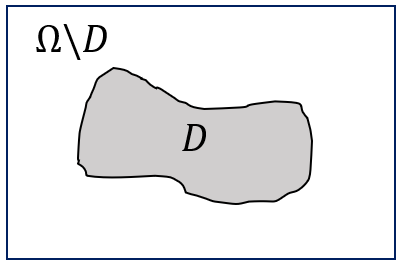
\includegraphics[width=0.375\linewidth]{image/sample-domain.png}
	\caption{$D$ แทนโดเมนต่อเติม}
	\label{figure:sample-domain}
\end{figure}

\hspace{1cm} การต่อเติมภาพเฉดเทาเป็นการหาค่าความเหมาะสมบนพื้นที่ได้รับความเสียหายที่อยู่บนภาพ $z$ ในบริเวณโดเมนต่อเติม $D$ โดยใช้ข้อมูลที่มีอยู่ใน $\Omega \textbackslash D$ เพื่อหาค่าเหมาะสมที่สุดบน $D$ 

\subsection{การนำเสนอภาพสี}

\hspace{1cm} ต่อไปจะพิจารณาภาพสี $\boldsymbol{I}$ ในระบบ RGB นั่นคือ เราพิจารณาว่าภาพ $\boldsymbol{u}$ ประกอบด้วยสี 3 สี คือ สีแดง, สีเขียว และสีน้ำเงิน จึงเขียนภาพ $\boldsymbol{I}$  ในรูปแบบของเวกเตอร์ โดยนิยาม
\begin{align*}
	\boldsymbol{I} = (I_1,I_2,I_3)^{\top} : \Omega  \rightarrow V^3	
\end{align*}

\noindent เมื่อ $I_1,I_2,I_3: \Omega  \rightarrow V$ แทนภาพในเฉดสีแดง สีเขียว และสีน้ำเงิน ซึ่งการต่อเติมภาพสีที่พูดถึงในโครงงานวิจัยนี้จะทำการแยกแต่ละเฉดสีออกเป็นเฉดเทา 3 ระนาบ แล้วจึงใช้การต่อเติมภาพเฉดเทากับทั้ง 3 เฉดสีก่อนรวมกลับเป็นภาพสีอีกครั้ง

